\documentclass[11pt]{article}

\usepackage[margin=1in]{geometry}
\usepackage{booktabs}
\usepackage{tabularx}
\usepackage{array}
\usepackage{graphicx}
\usepackage{subcaption}
\usepackage{siunitx}
\usepackage{enumitem}
\usepackage{amsmath}
\usepackage{hyperref}
\usepackage{float}

\sisetup{
  round-mode=places,
  round-precision=4,
  detect-all=true
}

\title{Agentic Influenza Model Discovery:\\Experiments and Results Draft}
\author{}
\date{\today}

\begin{document}

\maketitle

\begin{abstract}
This draft captures the current experimental and empirical core of
\texttt{agentic\_flu\_model\_discovery}. The benchmark compares deterministic,
probabilistic, fractional, hospitalization-aware, and delayed-observation
manual baselines against a constrained non-LLM discovery loop over epidemic
structure and observation maps. The current evidence supports age-aware model
selection under structural and observation uncertainty rather than a single
globally dominant model family.
\end{abstract}

\tableofcontents

\section{Introduction}

Weekly influenza hospitalization forecasting sits at an awkward intersection
between mechanistic epidemiology and operational prediction. On one hand,
compartmental epidemic models remain attractive because they offer interpretable
latent states, controllable inductive bias, and explicit constraints such as
non-negativity and approximate mass conservation. On the other hand, practical
forecast targets such as hospitalization rate are not observed directly as
canonical infectious prevalence. A model can therefore fail not only because
its latent disease dynamics are misspecified, but also because its
\emph{observation semantics} are mismatched to the public-health quantity being
predicted.

This mismatch is especially relevant for a proof-of-concept benchmark based on
a single FluSurv-NET season. In such a setting, one should not expect a single
model family to dominate across all age strata. Different age groups may differ
in latency, effective susceptibility recycling, reporting delay, and the extent
to which observed hospitalization rates align with latent infectious burden.
Accordingly, the central scientific question is not simply which model wins on
one leaderboard, but rather:
\begin{quote}
Can a constrained, fully programmatic structure-discovery loop identify when
simple mechanistic baselines are sufficient and when alternative latent or
observation structures become useful?
\end{quote}

This repository deliberately answers that question without placing a language
model inside the fitting loop. The current benchmark treats the ``agentic''
component as a propose-fit-verify-refine search procedure over a small grammar
of epidemic structures and observation maps. Candidate models are generated
programmatically, screened for biological and structural validity, fitted with
multiple random restarts, scored on validation and rolling-origin behavior, and
refined through beam search. This design makes the non-LLM control condition
strong enough to support a later LLM-based extension without confusing search
automation with semantic reasoning.

The benchmark evolved in three substantive steps. First, it established a
reproducible non-LLM forecasting core spanning deterministic, probabilistic,
and fractional SEIR baselines together with constrained structure discovery.
Second, it strengthened the comparison set with fair hospitalization-aware
manual baselines and benchmark-level conformal uncertainty post-processing.
Third, it elevated observation structure to a first-class discovery object by
allowing delayed infectious observation and hospitalization-aware observation
maps inside the search grammar. This last step matters because the target is a
hospitalization-rate series: if discovery is allowed to vary only latent
compartments while the observation map remains effectively fixed, then the
comparison between hand-designed and discovered models is incomplete.

The main empirical outcome is now clear. The benchmark does \emph{not} support
a single globally dominant model family. Instead, it supports
\emph{age-aware model selection under structural and observation uncertainty}.
In the current five-seed observation-aware benchmark:
\begin{itemize}[leftmargin=1.5em]
\item constrained discovery is a stable success case for the \texttt{0--4 yr}
series;
\item stronger manual baselines dominate or match discovery for
\texttt{Overall}, \texttt{18--49 yr}, and \texttt{50--64 yr};
\item delayed infectious observation emerges repeatedly in children and older
adults;
\item direct hospitalization observation is not selected by discovery in the
current single-season benchmark; and
\item removing the age prior does not change the selected structures,
observation maps, delays, or aggregate discovery errors.
\end{itemize}

These results turn the repository into a strong non-LLM experimental core for a
subsequent LLM phase. Because the current benchmark already contains fair manual
baselines, observation-aware discovery, multi-seed robustness analysis,
benchmark-level uncertainty calibration, and no-age-prior ablations, the next
step can focus narrowly on whether an LLM improves candidate proposal and
critique efficiency rather than on whether the underlying fitting and
evaluation pipeline is sound.

\section{Method}

\subsection{Benchmark objective}

The benchmark is designed to compare mechanistic model families for weekly
influenza hospitalization-rate forecasting under a common data-processing,
fitting, and evaluation protocol. The objective is twofold:
\begin{enumerate}[leftmargin=1.5em]
\item quantify point-forecast and uncertainty performance across manual and
discovered epidemic models; and
\item determine whether constrained non-LLM structure discovery provides
useful age-specific latent or observation structures beyond strong hand-designed
baselines.
\end{enumerate}

The benchmark treats all epidemic states in normalized population units and
keeps the total latent population approximately conserved through explicit
penalties. All models expose a single observation scaling coefficient $\rho$ so
that the benchmark compares latent disease dynamics and observation semantics
rather than arbitrary output rescaling tricks.

\subsection{Data processing and series construction}

The raw FluSurv-NET CSV is read with \texttt{skiprows=2} to discard metadata
lines above the table. Rows with missing \texttt{WEEK} or \texttt{YEAR.1} are
removed, the remaining rows are sorted chronologically by year and week, and a
continuous integer time index $t \in \{0, \dots, T-1\}$ is created. The primary
series is the \emph{Entire Network} / \emph{Overall} weekly rate. Robustness is
evaluated on five age-stratified series:
\texttt{0--4 yr}, \texttt{5--17 yr}, \texttt{18--49 yr},
\texttt{50--64 yr}, and \texttt{$\geq$65 yr}.

\subsection{Manual model families}

\paragraph{Deterministic SEIR.}
The deterministic baseline uses seasonal transmission
\[
\beta_t = \operatorname{softplus}\!\left(b_0 +
b_1 \sin(2 \pi t / 52) + b_2 \cos(2 \pi t / 52)\right)
\]
with discrete latent dynamics over $(S,E,I,R)$ and observation model
$\hat{y}_t = \rho I_t$. Trainable parameters include the seasonal coefficients,
transition rates, observation scale, and initial exposed/infectious mass.

\paragraph{Probabilistic SEIR.}
The probabilistic baseline shares the same latent dynamics but replaces the
deterministic observation equation with a Student-$t$ observation model. The
benchmark fits this model by MAP estimation and then constructs bootstrap-based
raw predictive intervals. Point forecasts are the bootstrap centers; interval
calibration is handled later as benchmark-level post-processing.

\paragraph{Fractional SEIR.}
The fractional baseline extends SEIR with a shared order parameter
$\alpha \in [0.7, 1.0]$ and a discrete memory approximation. The intent is to
test whether long-memory latent dynamics provide stable forecasting benefit for
the hospitalization-rate target.

\paragraph{Hospitalized SEIHR.}
The hospitalization-aware manual baseline uses five compartments
$(S,E,I,H,R)$ with both direct recovery and hospitalization pathways:
\[
S \rightarrow E \rightarrow I,\qquad
I \rightarrow R,\qquad
I \rightarrow H \rightarrow R.
\]
Its weekly discrete dynamics are
\begin{align*}
S_{t+1} &= S_t - \beta_t S_t I_t, \\
E_{t+1} &= E_t + \beta_t S_t I_t - \sigma E_t, \\
I_{t+1} &= I_t + \sigma E_t - \eta I_t - \gamma_i I_t, \\
H_{t+1} &= H_t + \eta I_t - \gamma_h H_t, \\
R_{t+1} &= R_t + \gamma_i I_t + \gamma_h H_t,
\end{align*}
with observation model $\hat{y}_t = \rho H_t$. This corrected specification
avoids forcing every infectious individual through the hospitalized compartment.

\paragraph{Delayed-observation SEIR.}
This baseline preserves the standard SEIR latent dynamics but changes the
observation equation to
\[
\hat{y}_t = \rho I_{t-d}, \qquad d \in \{0,1,2,3\},
\]
where the delay $d$ is selected by validation MAE only. This model isolates the
contribution of observation delay without changing the latent epidemic process.

\subsection{Constrained structure discovery}

The discovery module searches over a bounded grammar rather than over arbitrary
symbolic dynamics. A structure specification contains:
\begin{itemize}[leftmargin=1.5em]
\item a compartment template from
\{\texttt{SIR}, \texttt{SEIR}, \texttt{SEIRS}, \texttt{SEIHR}, \texttt{SEIAR}\},
\item a fractional on/off flag,
\item an observation map from
\{\texttt{I}, \texttt{H}, \texttt{I+H}, \texttt{delayed\_I}\}, and
\item a delay parameter in $\{0,1,2,3\}$ when the observation map is
\texttt{delayed\_I}.
\end{itemize}

The search begins from \texttt{SEIR} and iterates a
propose-fit-verify-refine loop:
\begin{enumerate}[leftmargin=1.5em]
\item fit the current candidate;
\item generate one-hop neighbors via structure edits, observation-map edits,
fractional toggles, and delay edits;
\item reject invalid candidates using structural validity rules;
\item fit all remaining candidates with multiple random restarts;
\item score candidates using validation and rolling-origin criteria plus
complexity penalties; and
\item retain the top beam until convergence or early stopping.
\end{enumerate}

Validity rules enforce that infection originates from $S$, infectious-like
states eventually reach recovery, no isolated compartments exist, and
observation semantics are compatible with the latent template. For example,
\texttt{obs=H} and \texttt{obs=I+H} require an $H$ compartment, while
\texttt{obs=delayed\_I} requires an $I$ compartment and a valid delay.

To keep search tractable, delayed-observation neighbors are only introduced
from \texttt{SIR}, \texttt{SEIR}, and \texttt{SEIRS}; observation-map
neighbors for \texttt{SEIHR} prioritize \texttt{I}, \texttt{H}, and
\texttt{I+H}; and the maximum number of compartments remains capped at five.

\subsection{Discovery scoring}

Discovery is selected by a stability-aware score that combines predictive
quality and structural parsimony. At a high level, candidates are penalized for
\begin{itemize}[leftmargin=1.5em]
\item validation MAE,
\item rolling-origin error and stability,
\item additional free parameters,
\item additional compartments,
\item observation-map complexity,
\item delayed observation length, and
\item optional age-specific structural priors.
\end{itemize}

This design intentionally favors structures that are not only accurate on one
validation segment but also stable across rolling-origin forecasts. The age
prior can be toggled on or off as an explicit ablation, and the current
multi-seed observation-aware reruns show identical results with and without it.

\subsection{Benchmark-level uncertainty calibration}

Raw predictive intervals are produced only by the probabilistic SEIR model.
They are then calibrated \emph{after} benchmarking via a benchmark-level
post-processing pipeline. Five calibration kinds are compared:
\texttt{raw}, \texttt{scale\_calibrated}, \texttt{conformal\_absolute},
\texttt{conformal\_standardized}, and \texttt{conformal\_asymmetric}. Method
selection is based strictly on validation, never on test labels.

The current default uncertainty postprocessor is the balanced conformal
winner-selection rule \texttt{v3}, which trades a very small increase in
absolute coverage gap relative to the most coverage-oriented rule for visibly
better interval score and narrower widths.

\subsection{Robustness and ablations}

The current non-LLM evidence base includes:
\begin{itemize}[leftmargin=1.5em]
\item five-seed robustness analysis over seeds
$\{0,1,2,42,2024\}$,
\item a single-seed age-prior ablation,
\item an observation-aware five-seed no-age-prior ablation, and
\item conformal winner-rule comparison.
\end{itemize}

Together these controls allow us to separate three questions:
\begin{enumerate}[leftmargin=1.5em]
\item whether discovery wins are stable across optimization randomness;
\item whether delayed observation arises from data and the search objective
rather than from the age prior; and
\item whether probabilistic intervals can be calibrated without contaminating
point-forecast evaluation.
\end{enumerate}

\section{Experiments}

\subsection{Data and forecasting task}

We study weekly influenza hospitalization-rate forecasting using a
FluSurv-NET CSV export. The benchmark reads the raw file with
\texttt{skiprows=2}, removes non-tabular disclaimer rows with missing
\texttt{WEEK} or \texttt{YEAR.1}, sorts chronologically by year and week, and
creates a continuous time index. The primary target series is the weekly
hospitalization rate for the \emph{Entire Network} catchment with all other
metadata fields set to \emph{Overall}. We also evaluate five age-stratified
series: \texttt{0-4 yr}, \texttt{5-17 yr}, \texttt{18-49 yr},
\texttt{50-64 yr}, and \texttt{>= 65 yr}.

All epidemic models operate in normalized population units with latent
compartment states summing approximately to one, except for numerical
deviations controlled by explicit mass-conservation penalties.

\subsection{Chronological splits and metrics}

For each series, we use a chronological split with the first $60\%$ of weeks
for training, the next $20\%$ for validation, and the last $20\%$ for test.
In addition to fixed held-out test evaluation, we run rolling-origin
forecasting at horizons $1$, $2$, and $4$ weeks ahead.

Point-forecast evaluation uses:
\begin{itemize}[leftmargin=1.5em]
\item mean absolute error (MAE),
\item root mean squared error (RMSE), and
\item sMAPE.
\end{itemize}

For probabilistic forecasts, we also track negative log-likelihood, empirical
interval coverage, average interval width, and interval score. Uncertainty
calibration is handled separately at the benchmark level and does not modify
point forecasts.

\subsection{Model families}

The benchmark currently compares six model families:
\begin{enumerate}[leftmargin=1.5em]
\item \texttt{deterministic\_seir}: a seasonal discrete-time SEIR baseline with
observation model $\hat{y}_t = \rho I_t$.
\item \texttt{probabilistic\_seir}: the same latent dynamics with Student-$t$
observations and bootstrap-based uncertainty.
\item \texttt{fractional\_seir}: a fractional-order extension with shared order
$\alpha \in [0.7, 1.0]$.
\item \texttt{hospitalized\_seihr}: a hospitalization-aware baseline with
compartments $(S,E,I,H,R)$ and observation model $\hat{y}_t = \rho H_t$.
\item \texttt{delayed\_observation\_seir}: standard SEIR dynamics with delayed
observation $\hat{y}_t = \rho I_{t-d}$, where $d \in \{0,1,2,3\}$ is chosen by
validation MAE only.
\item \texttt{constrained\_structure\_discovery}: a non-LLM propose-fit-verify-
refine search over a small epidemic grammar.
\end{enumerate}

The manual \texttt{hospitalized\_seihr} baseline was corrected in the current
round to allow both direct recovery $I \rightarrow R$ and hospitalization
$I \rightarrow H \rightarrow R$, rather than forcing every infectious
individual through the hospitalized compartment.

\subsection{Observation-aware constrained discovery}

The discovery procedure searches over both latent structure and observation
semantics. The allowed compartment templates are:
\[
\texttt{SIR}, \texttt{SEIR}, \texttt{SEIRS}, \texttt{SEIHR}, \texttt{SEIAR}.
\]

The current grammar also supports:
\begin{itemize}[leftmargin=1.5em]
\item a fractional toggle,
\item observation maps \texttt{I}, \texttt{H}, \texttt{I+H}, and
\texttt{delayed\_I},
\item observation delays of $1$, $2$, or $3$ weeks for
\texttt{delayed\_I}.
\end{itemize}

Structural validity rules enforce biologically plausible infection flow,
eventual recovery, no isolated compartments, and compatibility between
observation maps and available compartments. For example, \texttt{obs=H} and
\texttt{obs=I+H} are only valid when an $H$ compartment exists, while
\texttt{obs=delayed\_I} requires an $I$ compartment.

The discovery loop is programmatic rather than language-model-driven. Starting
from \texttt{SEIR}, the procedure repeatedly:
\begin{enumerate}[leftmargin=1.5em]
\item proposes one-hop neighbors,
\item validates each candidate structure,
\item fits valid candidates,
\item scores them on validation and rolling-origin behavior,
\item retains the top beam, and
\item stops early when the search stagnates.
\end{enumerate}

To keep the search space controlled, delayed-observation neighbors are only
generated from \texttt{SIR}, \texttt{SEIR}, and \texttt{SEIRS}, while
\texttt{SEIHR} candidates prioritize \texttt{obs=I}, \texttt{obs=H}, and
\texttt{obs=I+H}. Complexity scoring includes penalties for additional free
parameters, compartments, recurrence, fractional order, observation-map
complexity, and delayed observation length.

\subsection{Seeds, robustness, and ablations}

The main robustness analysis uses five seeds:
\[
\{0, 1, 2, 42, 2024\}.
\]
For each seed, we rerun the full age-stratified benchmark and aggregate mean
performance, standard deviations, and win rates.

We also ran two ablations relevant to the current paper narrative.

\paragraph{Age-prior ablation.}
The discovery score contains an optional age-specific prior over structure
families. A single-seed age-prior ablation and a five-seed observation-aware
no-age-prior rerun both showed identical selected structures and identical
aggregate model summaries relative to the age-prior-enabled run. In the
observation-aware multi-seed setting, the ablation also leaves the dominant
observation map and dominant delay mode unchanged for every series. This
strongly suggests that the current discovery patterns are not being trivially
forced by the age prior.

\paragraph{Benchmark-level conformal calibration.}
Probabilistic interval calibration is handled as a separate benchmark-level
post-processing step, not inside model fitting. Five calibration kinds are
compared (\texttt{raw}, \texttt{scale\_calibrated},
\texttt{conformal\_absolute}, \texttt{conformal\_standardized},
\texttt{conformal\_asymmetric}), and calibration-method selection is based on
validation only. The current default winner-selection rule is the balanced
\texttt{v3} rule, which preserves nearly the same coverage gap as the most
coverage-oriented rule while reducing interval score and width.

\subsection{Implementation details}

All models use multiple random restarts and explicit penalties for negative
states and mass-conservation violations. The current age-robustness benchmark
uses six restarts for each train fit, one restart for rolling-origin refits,
and a maximum of 250 optimization iterations per restart. The discovery beam
width is five, the maximum number of rounds is twenty, and search uses both
validation MAE and rolling-origin stability criteria. The codebase is fully
tested, with plain \texttt{pytest -q} supported via a repository-level
\texttt{pytest.ini}.

\subsection{LLM-guided comparison protocol}

The repository now contains two LLM-facing layers that sit on top of the
existing non-LLM benchmark rather than replacing it.

\paragraph{LLM-V0.}
LLM-V0 is a proposal-only layer. It constructs a prompt-safe series summary,
adds a static hospitalization-semantics card, asks a proposer for JSON
structure candidates, asks a critic for annotations, applies the same hard
validator used by the non-LLM discovery pipeline, and then evaluates all
hard-valid candidates with the existing numerical executor. It therefore tests
whether proposal parsing, leakage guards, hard validation, and non-LLM
executor reuse all work end-to-end.

\paragraph{LLM-V1.}
LLM-V1 adds iterative refinement. Round 1 matches V0:
\[
\texttt{summary} \rightarrow \texttt{semantics} \rightarrow
\texttt{proposer} \rightarrow \texttt{critic} \rightarrow
\texttt{hard validator} \rightarrow \texttt{executor}.
\]
For rounds $r \geq 2$, a result analyst reads only validation- and
rolling-derived outputs from round $r-1$ and emits bounded feedback for the
next proposer call. The proposer is then restricted to small edits around the
previous best candidate, after which the critic, hard validator, and executor
run again.

\paragraph{Comparison design.}
The intended LLM comparison is three-way:
\begin{enumerate}[leftmargin=1.5em]
\item \textbf{LLM-V0}: one-shot proposal-only search;
\item \textbf{LLM-V1}: iterative validation-feedback refinement; and
\item \textbf{non-LLM constrained discovery}: the observation-aware discovery
baseline already used throughout the repository.
\end{enumerate}

This comparison is not meant to ask only whether the LLM achieves a lower test
MAE. Instead, it asks whether an agentic refinement loop improves proposal
quality, semantic alignment, and validation-selected candidate quality under
the same mechanistic constraints and executor.

\paragraph{Prompt-safe inputs and no-test leakage.}
All LLM-facing inputs are built from prompt-safe summaries. The proposer,
critic, and analyst are not allowed to see:
\begin{itemize}[leftmargin=1.5em]
\item held-out test metrics such as \texttt{test\_mae}, \texttt{test\_rmse},
or \texttt{test\_smape},
\item best-test model identifiers,
\item test-policy recommendations, and
\item test-winner files such as \texttt{benchmark\_series\_winners}.
\end{itemize}
Allowed prompt content includes only series identity, training summary,
validation summary, rolling validation summary, surveillance semantics, current
non-test discovery structure modes, and previous-round validation/rolling
feedback. Held-out test metrics are computed only after the final
validation/rolling-selected candidate is fixed.

\paragraph{Evaluation metrics.}
The LLM protocol tracks six classes of outputs:
\begin{itemize}[leftmargin=1.5em]
\item \textbf{valid proposal rate}: fraction of raw proposals that become
hard-valid candidates;
\item \textbf{candidate efficiency}: number of evaluated candidates relative to
the non-LLM reference search budget;
\item \textbf{best validation score}: the best composite
validation/rolling-oriented discovery score reached in the run;
\item \textbf{rolling validation MAE}: the mean rolling-origin validation MAE
of the selected candidate;
\item \textbf{selected-candidate test MAE}: held-out test MAE computed only
after the final validation-selected candidate is fixed; and
\item \textbf{semantic alignment}: whether proposed observation maps are
consistent with the hospitalization-rate target.
\end{itemize}
Efficiency claims are explicitly suppressed unless the LLM and non-LLM budgets
are matched.

\paragraph{Provider distinction.}
The LLM stack now supports both \texttt{provider=mock} and
\texttt{provider=openai}. The mock provider is used for engineering validation:
schema enforcement, leakage guards, round-aware artifact generation, and
executor reuse. Live-provider runs are the appropriate setting for scientific
evaluation, but only after the resulting artifacts are validated and frozen
under the same protocol. The currently frozen repository artifacts remain
mock-provider engineering runs.

\section{Results}

\subsection{Main empirical takeaway}

The strongest overall conclusion is not that one model family wins everywhere.
Instead, the benchmark supports \emph{age-aware model selection under
structural and observation uncertainty}. Strong hand-designed baselines remain
competitive or superior for several series, while constrained discovery is
clearly useful for selected age groups. Observation structure also matters:
once the discovery grammar is allowed to search over delayed observation, it
selects \texttt{delayed\_I} in multiple age groups, but it still does not
select \texttt{H} or \texttt{I+H} in the current single-season benchmark.

\subsection{Observation-aware multi-seed point-forecast results}

Table~\ref{tab:obs-aware-summary} summarizes the current observation-aware
five-seed aggregate. The table is based on
\texttt{artifacts\_multiseed\_age\_robustness\_observation/} and reflects the
latest non-LLM control benchmark.

\begin{table}[H]
\centering
\caption{Observation-aware five-seed recommendation summary. The
recommendation column reports the modal recommendation over seeds, while the
``best test'' and ``best rolling'' columns summarize which model family most
often wins the held-out test split and rolling-origin evaluation.}
\label{tab:obs-aware-summary}
\begin{tabularx}{\textwidth}{>{\raggedright\arraybackslash}p{1.45cm} >{\raggedright\arraybackslash}p{3.0cm} >{\raggedright\arraybackslash}p{2.7cm} >{\raggedright\arraybackslash}p{2.7cm} X}
\toprule
Series & Recommended model & Best test pattern & Best rolling pattern & Interpretation \\
\midrule
Overall & \texttt{deterministic\_seir} & \texttt{delayed\_observation\_seir} wins $4/5$ seeds & split between deterministic and delayed baselines & Observation-aware manual baselines dominate discovery on the overall aggregate. \\
0--4 yr & \texttt{constrained\_structure\_discovery} & discovery wins $5/5$ seeds & discovery wins $5/5$ seeds & Clearest stable discovery success case in the repository. \\
5--17 yr & \texttt{constrained\_structure\_discovery} & discovery wins $4/5$ seeds & \texttt{probabilistic\_seir} wins $5/5$ seeds & Strong held-out discovery result, but rolling-origin stability still favors the probabilistic baseline. \\
18--49 yr & \texttt{deterministic\_seir} & split across deterministic, delayed, and hospitalized baselines & deterministic wins $3/5$ seeds & Discovery is not competitive; the relevant comparison is among strong manual baselines. \\
50--64 yr & \texttt{delayed\_observation\_seir} & \texttt{hospitalized\_seihr} wins $3/5$ seeds & delayed baseline wins $4/5$ seeds & Fair hospitalization-aware baselines largely replace discovery as the main story. \\
$\geq$65 yr & \texttt{deterministic\_seir} & deterministic wins $3/5$ seeds & discovery wins $4/5$ seeds & The older-adult series remains split-sensitive between held-out and rolling-origin criteria. \\
\bottomrule
\end{tabularx}
\end{table}

The numerical aggregate reinforces this qualitative view. For the overall
series, \texttt{delayed\_observation\_seir} achieves mean test
MAE~\num{0.035056}, outperforming \texttt{deterministic\_seir}
(\num{0.035205}) and discovery (\num{0.036967}). For \texttt{0-4 yr},
discovery remains decisively best with mean test MAE~\num{0.090596} and mean
rolling MAE~\num{0.123344}. In contrast, for \texttt{50-64 yr},
\texttt{hospitalized\_seihr} wins held-out test most often while
\texttt{delayed\_observation\_seir} dominates rolling-origin MAE, making this
age group far less of a clean discovery-wins case than it appeared before the
fair-baseline expansion.

\begin{figure}[H]
\centering
\begin{subfigure}[t]{0.49\textwidth}
  \centering
  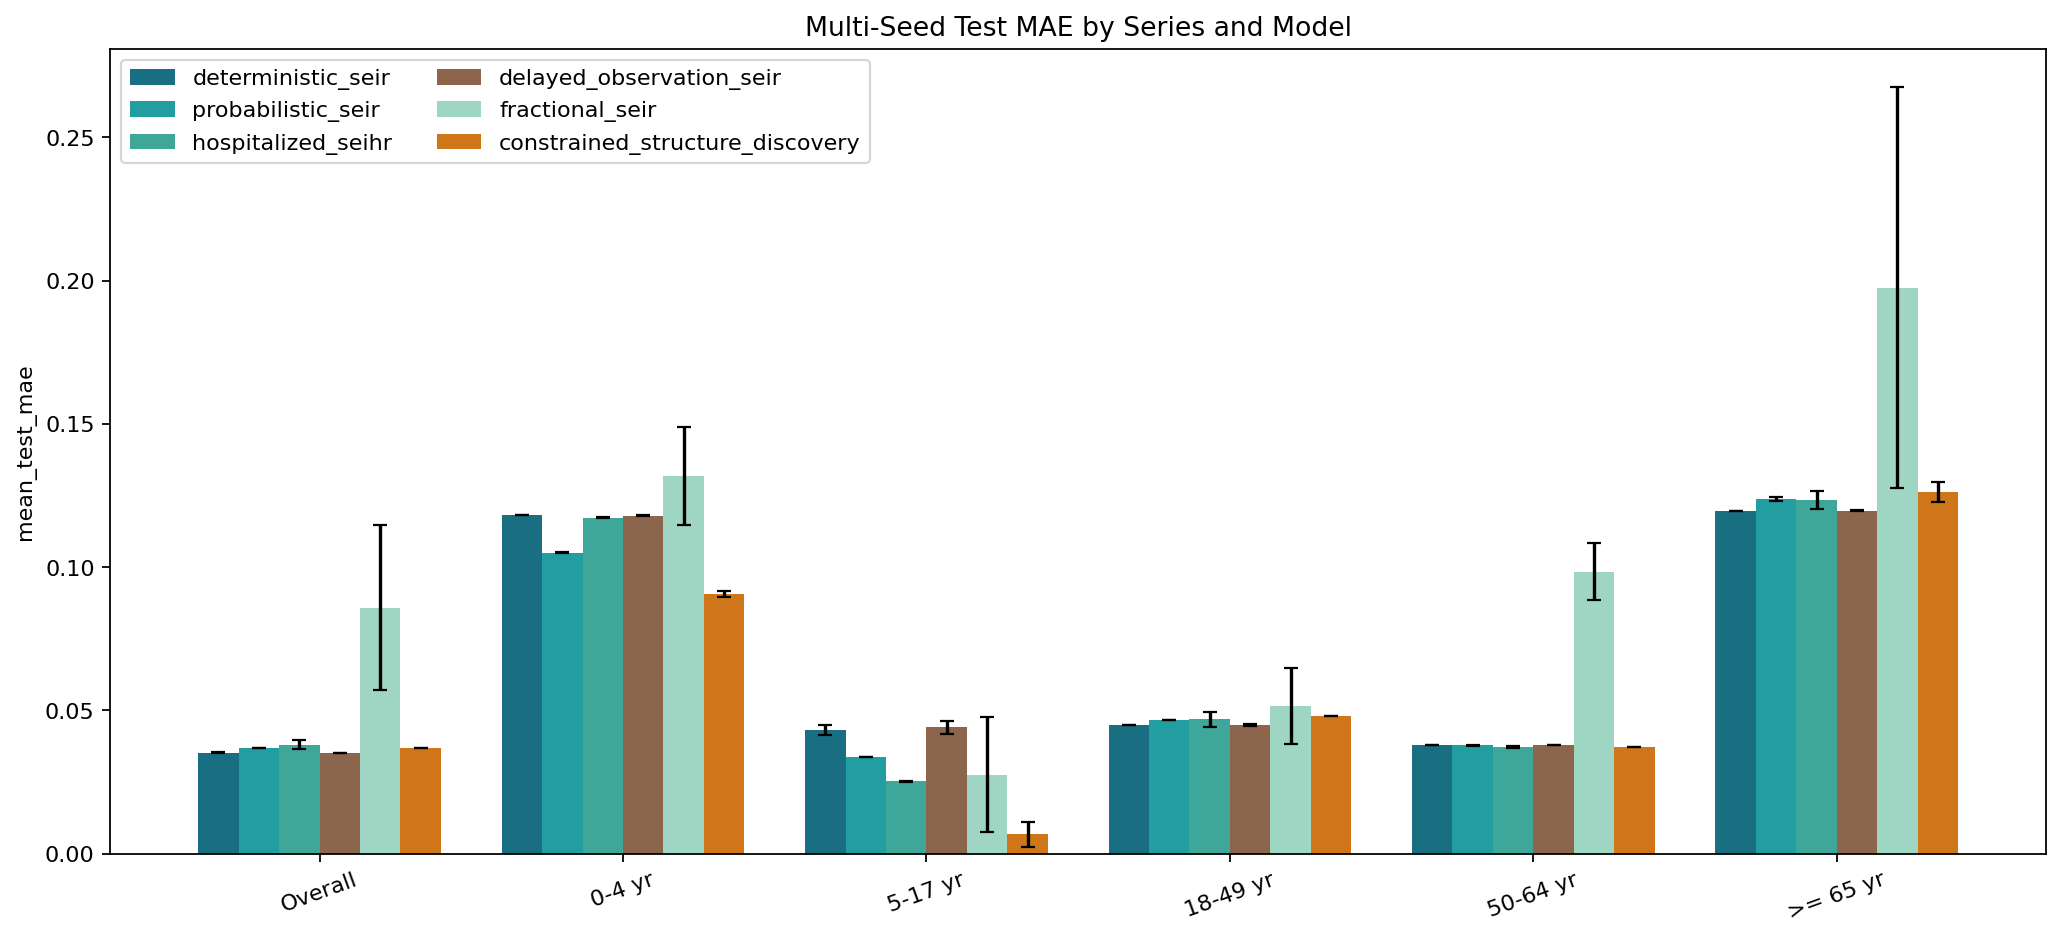
\includegraphics[width=\linewidth]{../artifacts_multiseed_age_robustness_observation/multiseed_test_mae_errorbars.png}
  \caption{Held-out test MAE across five seeds.}
\end{subfigure}
\hfill
\begin{subfigure}[t]{0.49\textwidth}
  \centering
  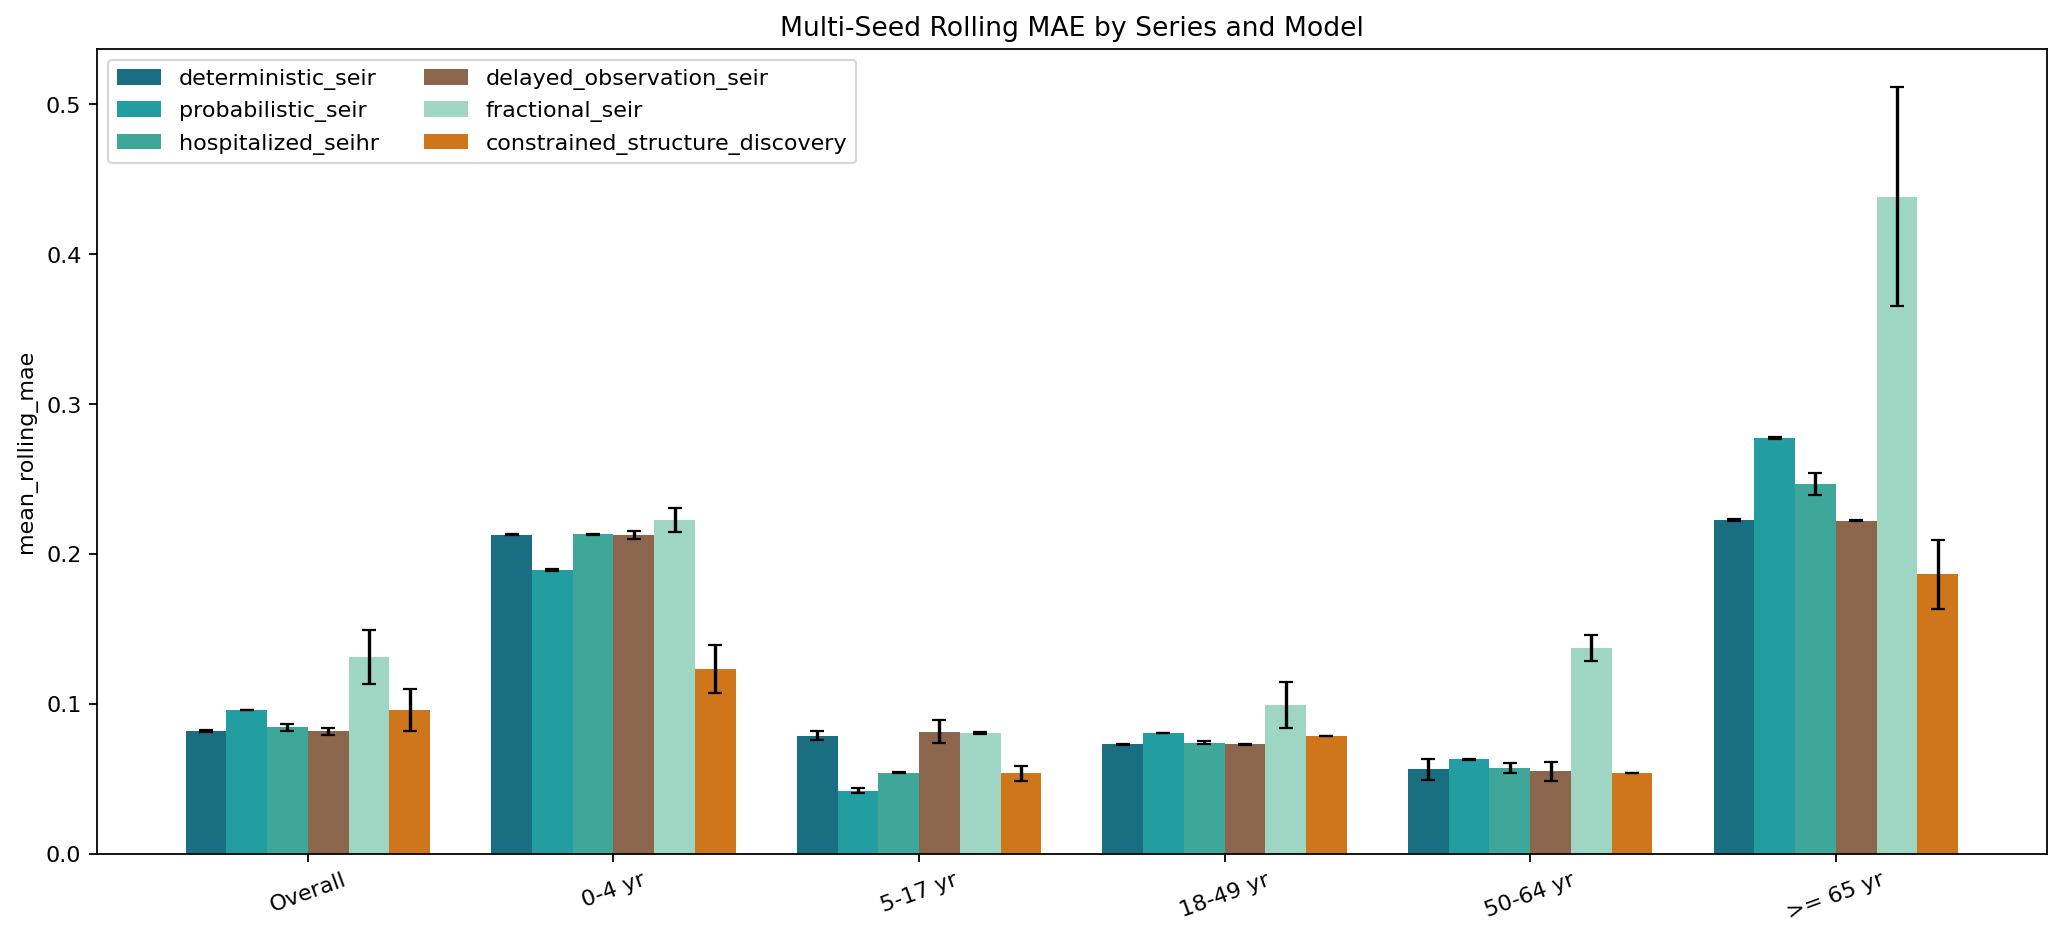
\includegraphics[width=\linewidth]{../artifacts_multiseed_age_robustness_observation/multiseed_rolling_mae_errorbars.png}
  \caption{Rolling-origin MAE across five seeds.}
\end{subfigure}
\caption{Observation-aware five-seed robustness plots. Error bars summarize
between-seed variability.}
\label{fig:obs-aware-multiseed}
\end{figure}

\subsection{Objective-aware policy interpretation}

The five-seed aggregate also benefits from a tie-aware policy layer. Rather
than forcing a single recommendation whenever one mean error is numerically
smallest, we define a practical tie separately for held-out test MAE and
rolling-origin MAE:
\[
|m - m^\star| \leq \max(0.001, 0.02 m^\star),
\]
where $m^\star$ is the best mean metric for the current series and objective.
Within each tie set, models are ranked by win rate, between-seed variability,
parameter count, and simplicity priority. This produces
\texttt{test\_policy\_model}, \texttt{rolling\_policy\_model}, and, when
possible, a shared \texttt{parsimony\_policy\_model}.

This policy layer changes how the benchmark should be interpreted. It shows
that $4/6$ series have different held-out-test and rolling-origin policy
winners, but only two series remain fully objective-dependent with no shared
parsimonious compromise. The clean cases are still informative:
\texttt{0--4 yr} remains a discovery win under both objectives, while
\texttt{18--49 yr} collapses to a deterministic recommendation once practical
ties are acknowledged. More interestingly, \texttt{Overall} becomes a
practical tie between \texttt{deterministic\_seir} and
\texttt{delayed\_observation\_seir}, with the deterministic model preferred as
the simpler shared compromise. Likewise, \texttt{50--64 yr} has different test
and rolling winners, yet discovery remains inside both tie sets and therefore
survives as the parsimonious compromise even after fair hospitalization-aware
baselines are added.

The implication is that the current non-LLM benchmark should be described not
only as age-aware but also as objective-aware. Some series genuinely reward one
model over another, but several series are better interpreted as practical ties
whose final recommendation depends on whether the user prioritizes held-out
split accuracy, rolling-origin stability, or model simplicity.

\subsection{Discovery structure and observation semantics}

Table~\ref{tab:discovery-structures} summarizes the structures selected by the
observation-aware discovery grammar over five seeds.

\begin{table}[H]
\centering
\caption{Selected discovery structures in the observation-aware five-seed
benchmark. Frequencies are computed over the five random seeds.}
\label{tab:discovery-structures}
\begin{tabularx}{\textwidth}{>{\raggedright\arraybackslash}p{1.45cm} >{\raggedright\arraybackslash}p{4.4cm} >{\raggedright\arraybackslash}p{1.6cm} X}
\toprule
Series & Dominant selected structure(s) & Frequency & Interpretation \\
\midrule
Overall & \texttt{SIR|fractional=0|obs=I} & $1.0$ & Discovery stays simple when richer observation maps are unnecessary. \\
0--4 yr & \texttt{SEIRS|obs=I} plus delayed variants with delay $1$ and $2$ & $0.6$ for \texttt{obs=I}; $0.4$ delayed combined & Discovery remains structure-rich and occasionally uses delayed observation in children. \\
5--17 yr & \texttt{SEIRS} family with \texttt{obs=I}, \texttt{delayed\_I|delay=2}, and \texttt{delayed\_I|delay=3} & mixed & Discovery explores delay here, but the selected family remains SEIRS in every seed. \\
18--49 yr & \texttt{SIR|fractional=0|obs=I} & $1.0$ & Observation search does not force extra complexity for this adult group. \\
50--64 yr & \texttt{SIR|fractional=0|obs=I} & $1.0$ & Even after observation-grammar expansion, discovery selects the same simple latent structure. \\
$\geq$65 yr & \texttt{SEIRS|fractional=1|obs=delayed\_I|delay=2} and \texttt{SEIRS|fractional=1|obs=I} & $0.6$ delayed, $0.4$ \texttt{I} & Older adults are the strongest case where delayed observation emerges stably from discovery. \\
\bottomrule
\end{tabularx}
\end{table}

Two points are especially important.

\paragraph{Delayed observation emerges without LLMs.}
The expanded grammar now allows the non-LLM discovery loop to recover explicit
observation delay. In the current benchmark, \texttt{delayed\_I} is selected in
children and older adults, including $3/5$ seeds for the
$\geq$65-yr series.

\paragraph{Hospitalization observation is not selected.}
No selected discovery winner uses \texttt{obs=H} or \texttt{obs=I+H}. This
does not imply that hospitalization-aware observation is universally useless:
the manual \texttt{hospitalized\_seihr} baseline remains competitive in several
age groups. Rather, it means that in the current proof-of-concept season, the
non-LLM search finds stronger evidence for delayed infectious observation than
for directly observing the hospitalized compartment.

\subsection{Age-prior ablation}

The observation-aware no-age-prior multi-seed rerun produced the same:
\begin{itemize}[leftmargin=1.5em]
\item \texttt{multiseed\_model\_summary.csv},
\item \texttt{multiseed\_age\_group\_recommendation.csv}, and
\item \texttt{multiseed\_discovery\_structure\_frequency.csv}
\end{itemize}
as the corresponding age-prior-enabled run.

More concretely, the derived comparison tables show:
\begin{itemize}[leftmargin=1.5em]
\item no change in recommended model mode for any of the six series,
\item no change in dominant discovery structure for any series,
\item no change in dominant observation-map mode for any series,
\item no change in dominant delay mode for any series, and
\item zero difference in aggregate discovery test MAE and aggregate discovery
rolling MAE for all six series.
\end{itemize}

This result matters because it rules out a simple confound: the delayed
observation structures are not appearing merely because the search was given an
age-specific structural preference. Instead, the current evidence suggests that
the observation-aware discovery results are driven by the data and the
validation-based search objective rather than by the age prior.

\subsection{Uncertainty calibration}

Although the main emphasis of the current paper core is on point forecasting,
the uncertainty pipeline is already mature enough to report a stable default.
Benchmark-level conformal calibration compares five calibration kinds and three
validation-only winner rules. The current selected rule is the balanced
\texttt{v3} rule.

\begin{table}[H]
\centering
\caption{Comparison of validation-only conformal winner rules. Lower is better
for all three metrics.}
\label{tab:conformal-rules}
\begin{tabular}{lccc}
\toprule
Rule & Mean absolute coverage gap & Mean interval score & Mean width \\
\midrule
v1 & \num{0.189394} & \num{0.460618} & \num{0.451670} \\
v2 & \num{0.183838} & \num{0.484247} & \num{0.473100} \\
v3 & \num{0.184343} & \num{0.465319} & \num{0.456298} \\
\bottomrule
\end{tabular}
\end{table}

The practical interpretation is that v1 is too interval-score-driven, v2 is
too coverage-gap-driven, and v3 provides the best current compromise. This is
why the repository now treats benchmark-level conformal v3 as the default
uncertainty postprocessor while keeping point-forecast selection separate.

\subsection{Implications for the next phase}

These experiments tighten the non-LLM story substantially. We now have:
\begin{enumerate}[leftmargin=1.5em]
\item fair hospitalization-aware manual baselines,
\item observation-aware discovery grammar,
\item five-seed robustness analysis,
\item no-age-prior ablation showing the same aggregate result, and
\item a fixed benchmark-level conformal postprocessor.
\end{enumerate}

This means the next phase should not continue to micro-tune non-LLM search.
Instead, the most valuable next step is an \textbf{LLM-V0} experiment in which
the LLM only proposes and critiques candidate structures while the existing
Python pipeline continues to enforce validity, perform fitting, and evaluate
validation-time performance. The current observation-aware non-LLM benchmark is
now strong enough to serve as a credible control condition for that study.


\end{document}
